\documentclass[12pt]{article} % Clase de documento, tamaño de letra 12pt

% Paquetes importantes
\usepackage[utf8]{inputenc}   % Codificación de entrada UTF-8 para caracteres acentuados
\usepackage[T1]{fontenc}      % Codificación de salida para que el texto se vea bien en PDF
\usepackage[spanish]{babel}   % Traduce términos automáticos al español (ej. "Figura", "Resumen")

\usepackage{csquotes}         % Recomendado para manejar comillas y citas con biblatex
\usepackage{graphicx}         % Permite incluir imágenes con \includegraphics
\usepackage{setspace}         % Para controlar interlineado; APA pide interlineado doble
\usepackage{geometry}         % Controla los márgenes de la página (APA pide 1 pulgada = 2.54cm)
\usepackage[hidelinks]{hyperref}        % Habilita enlaces clicables en el PDF (tabla de contenido, referencias)
\usepackage[style=apa, backend=biber]{biblatex}  % Bibliografía con estilo APA 7 y gestor biber
\addbibresource{referencias.bib}  % Archivo con las referencias bibliográficas (formato .bib)

% Carga tu paquete personalizado que contiene el comando \imprimircaratula
\usepackage{caratula}

%para decorar el indice
\usepackage{tocloft} %Conectar los títulos con los números de página usando puntos
\renewcommand{\cftsecleader}{\cftdotfill{\cftdotsep}} %Esto  añadirá los "........" entre el título y la página.


% Define los márgenes recomendados por APA: 1 pulgada en todos lados
\geometry{letterpaper, margin=1in}

% Permite personalizar el formato de títulos (secciones y subsecciones)
\usepackage{titlesec}
% Define estilo para títulos de sección: tamaño grande y negrita
\titleformat{\section}{\normalfont\large\bfseries}{\thesection}{1em}{}
% Define estilo para títulos de subsección: tamaño normal y negrita
\titleformat{\subsection}{\normalfont\normalsize\bfseries}{\thesubsection}{1em}{}

% Define interlineado doble, que es requerido por APA
\doublespacing
\usepackage{float}

%para la tabla
\usepackage{pdflscape} %Para rotar la página
\usepackage{adjustbox} %Para redimensionar automáticamente el contenido
\usepackage{tabularx} %Para hacer que la tabla ocupe todo el ancho de la página usando columnas flexibles
\usepackage{array} % Para usar >{\centering\arraybackslash}
\usepackage[table,xcdraw]{xcolor} %Para darle color al encabezado
\definecolor{headerbg}{HTML}{D9E1F2} % Para definir un color de encabezado
\usepackage{multirow}      % Para combinar filas

%para personalizar el header
\usepackage{fancyhdr}           % Para encabezados y pies personalizados
\pagestyle{fancy}               % Activar fancyhdr para todas las páginas
\fancyhf{}                      % Limpia encabezados y pies por defecto
%\fancyhead[L]{J. Aulla; C. Arancibia} % Encabezado a la izquierda con las siglas
\fancyhead[R]{\thepage}
\renewcommand{\headrulewidth}{0pt} %quita la linea debajo de los nombres y numero de pagina



% Datos para título, autor y fecha (aunque no se usan porque tienes portada personalizada)
\title{Título del Documento en Formato APA 7}
\author{Nombre del Autor}
\date{\today}

\begin{document}

% Imprime la portada con el comando definido en tu paquete caratula.sty
\imprimircaratula

\begin{center}
    \vspace*{3cm} 
    \normalsize \textbf{DEDICATORIA} 
    \vspace{6cm}
\end{center}
\hspace{7.9cm}
\begin{minipage}{\dimexpr\textwidth-8cm}
    \textcolor{gray}{
        Le dedicamos este trabajo a nuestros familiares, amigos y compañeros, 
        quienes nos han ayudado a alcanzar nuestros objetivos, apoyándonos y 
        aconsejándonos en circunstancias poco favorables.
    }
\end{minipage}

\newpage

\begin{center}
    \vspace*{3cm} 
    \normalsize \textbf{AGRADECIMIENTOS} 
    \vspace{6cm}
\end{center}
\hspace{7.9cm}
\begin{minipage}{\dimexpr\textwidth-8cm}
    \textcolor{gray}{
        Expresamos nuestro sincero agradecimiento a nuestra docente guía, \textbf{Charles Dummar Camasca Macedo}, por su constante apoyo, orientación y dedicación durante el desarrollo de este proyecto.
    }
\end{minipage}

\newpage

% Tabla de contenidos automática
\tableofcontents
\newpage

\listoffigures
\newpage

% Resumen (abstract) con su propio entorno
\begin{abstract}

La empresa, dedicada a la comercialización de componentes de PC, atraviesa un proceso de expansión que ha incrementado el número de sedes y el volumen de operaciones. Sin embargo, el control de inventario continúa realizándose de forma manual en cuadernos físicos, lo que provoca registros incompletos o duplicados, demoras en la actualización de existencias, ausencia de información en tiempo real y alta exposición a pérdidas por extravío o deterioro del soporte. La falta de trazabilidad por número de serie y por ubicación dificulta la conciliación entre almacenes y puntos de venta, limita la detección de mermas y devoluciones y reduce la confiabilidad de los datos.

Frente a este contexto, se plantea el desarrollo de un sistema web de inventario centralizado, escalable y seguro, que provea visibilidad en tiempo real del stock en múltiples sucursales y garantice datos consistentes. La solución propuesta se fundamenta en una arquitectura de microservicios, con Spring Boot para el backend, Angular para el frontend y SQL Server como motor de base de datos, privilegiando la trazabilidad, la disponibilidad y la facilidad de mantenimiento. El proyecto se gestionará con Scrum, mediante sprints cortos y entregables incrementales (MVP temprano, pruebas unitarias e integración, despliegue progresivo), asegurando alineamiento continuo con las necesidades del negocio y una adopción ordenada por parte de los usuarios.


\end{abstract}
\newpage

% Sección Introducción
\section*{Introducción}
\addcontentsline{toc}{section}{Introducción}

Este proyecto propone implementar un sistema web de control de almacén centralizado y escalable para reemplazar la gestión manual en cuadernos que hoy provoca errores, baja trazabilidad por serie y ubicación, falta de información en tiempo real y riesgos de quiebres o sobreinventario; la solución—basada en microservicios con Spring Boot (backend), Angular (frontend) y SQL Server—incorpora control de entradas, salidas, transferencias y ajustes, trazabilidad por número de serie, niveles mínimos con alertas, reportes operativos y gerenciales, control de accesos por roles, auditoría e integración con compras y ventas, y se gestionará con Scrum para asegurar entregas incrementales; con ello se busca reducir errores, mejorar el cumplimiento de pedidos y optimizar el abastecimiento con decisiones soportadas en datos confiables; en el presente documento se explicará, en el Capítulo I, la problemática, el planteamiento del problema, los objetivos, la justificación técnica y social y el alcance/arquitectura de la solución; y, en el Capítulo II, el marco teórico, los modelos de inventario pertinentes y la metodología de desarrollo (Scrum) con sus elementos clave.

\newpage
% Inicio del primer Capítulo
\section*{\makebox[\linewidth][c]{Capítulo I}}
\addcontentsline{toc}{section}{Capítulo I}

% Descripción de la problemática
\subsection*{Descripción de la problemática}
\addcontentsline{toc}{subsection}{Descripción de la problemática}

Una empresa dedicada a la comercialización de componentes de PC está en plena expansión, con nuevas sedes en operación. Sin embargo, el almacén general aún controla el inventario de forma manual en un cuaderno, un método ineficiente que genera omisiones de datos, limita la disponibilidad oportuna de la información y aumenta el riesgo de pérdidas.

% Planteamiento del Problema
\subsection*{Planteamiento del Problema}
\addcontentsline{toc}{subsection}{Planteamiento del Problema}

Se plantea desarrollar una solución web de inventario centralizada y escalable que permita a la empresa gestionar de manera eficiente el stock de componentes de PC en múltiples sucursales, con visibilidad en tiempo real y datos consistentes. La plataforma debe unificar la información dispersa y acompañar el crecimiento del negocio sin perder precisión ni oportunidad en los registros.

La solución debe asegurar trazabilidad a nivel de producto y número de serie, control de entradas, salidas, transferencias y ajustes, definición de niveles mínimos con alertas de reposición, generación de reportes operativos y gerenciales, control de acceso por roles y registros de auditoría, además de integrarse con los procesos de compras y ventas. Con ello se busca reducir errores, mejorar el cumplimiento de pedidos, optimizar el abastecimiento y respaldar decisiones oportunas basadas en información confiable.

% Inicio de los objetivos
\subsection*{Objetivos}
\addcontentsline{toc}{subsection}{Objetivos}

% Inicio de los objetivos
\subsubsection*{General}
\addcontentsline{toc}{subsubsection}{General}

Desarrollar un sistema web para el Control de Almacén para una tiemda de componentes.

% Planteo de los especificos
\subsubsection*{especificos}  
\addcontentsline{toc}{subsubsection}{especificos}

\begin{itemize}
  \item Recopilar información del negocio
  \item Definir las nesecidades del negocio y alcance
  \item Realizar analisis tecnico y de viabilidad
  \item Realizar Modelado de Entidades y Arquitectura
  \item Diseño UX/UI y maquetado
  \item Planificar el Desarrollo del proyecto
  \item desarrollar los entregables para cliente
  \item Realizar pruebas unitaria e integracion
  \item desplegar la Solucion
\end{itemize}

% Inicio de la Justificación
\subsection*{Justificación}
\addcontentsline{toc}{subsection}{Justificación}

% Inicio de la Justificación tecnica
\subsubsection*{tecnica}
\addcontentsline{toc}{subsubsection}{tecnica}

  \begin{enumerate}
  \item Sql server(Motor de base de datos):
  \begin{itemize}
    \item CPU: x64, mínimo 1.4 GHz (recomendado: 2.5 GHz+).
    \item RAM: 4 GB mínimo (recomendado: 16–32 GB).
    \item Almacenamiento: 6 GB libres (preferible SSD de 100 GB+).
    \item Sistema operativo: Windows Server 2016+ o Windows 10 1607+.
    \item Conectividad: Puerto 1433, codificación UTF-8, acceso vía JDBC
  \end{itemize}
  \item Spring Boot (Backend Java):
  \begin{itemize}
    \item CPU: 2 núcleos mínimo (recomendado: 4–8 núcleos).
    \item RAM: 4 GB mínimo (recomendado: 8–16 GB).
    \item Almacenamiento: 10 GB libres (preferible SSD).
    \item Java: Versión 17+.
    \item Sistema operativo: Windows 10+, Linux Ubuntu 20.04+.
    \item Dependencias: Spring Web, Spring Data JPA, Spring Security (opcional).
    \item Conexión: JDBC a SQL Server, configuración CORS para Angular.
  \end{itemize}
  \item Angular (Frontend TypeScript):
  \begin{itemize}
    \item CPU: 2 núcleos mínimo.
    \item RAM: 4 GB mínimo.
    \item Almacenamiento: 5 GB libres.
    \item Node.js: v18+.
    \item Sistema operativo: Windows, macOS o Linux.
    \item Producción: Archivos estáticos servidos por Nginx, Apache o CDN.
  \end{itemize}
\end{enumerate}

La Arquitectura para el Sistema de Control de Almacen se fundamenta en estas 3 tecnologias clave, estas responden a criterios de escalabilidad, trazabilidad, seguridad y facilidad de mantenimiento, alineados con los objetivos del negocio, por lo que el cliente a aprobado estos requerimientos.



% Inicio de la Justificación Social
\subsubsection*{Social}
\addcontentsline{toc}{subsubsection}{Social}

La implementación del sistema optimiza el trabajo interno al agilizar la búsqueda de productos y reducir errores, estandarizando procedimientos y disminuyendo el estrés operativo. Para las personas clientes, garantiza la disponibilidad por sucursal, acelera la atención y reduce las ventas fallidas, fortaleciendo la confianza en garantías y devoluciones. Además, impulsa la transformación digital de la empresa y deja el camino listo para integrar, en el futuro, un canal de e-commerce o una plataforma de soporte para sus clientes.
% Inicio de la Justificación Financiera
\subsubsection*{Financiera}
\addcontentsline{toc}{subsubsection}{Financiera}

La implementación del sistema de inventario es una inversión con retorno comprobable: la TIR proyectada es del 20\%, superior a la tasa de descuento exigida del 12\%, por lo que el proyecto resulta atractivo. En la operación, reduce pérdidas por errores de inventario y mermas, disminuye ventas fallidas y protege el capital de trabajo. La automatización de reportes y alertas de stock optimiza el uso del personal al liberar horas administrativas. La visibilidad en tiempo real y los tableros de BI mejoran la toma de decisiones sobre compras, reposición y transferencias, elevando la rotación saludable y reduciendo el sobreinventario. Además, la arquitectura de microservicios con despliegue contenedorizado garantiza escalabilidad: permite agregar nuevos módulos sin invertir en más hardware y con costos predecibles. En conjunto, la solución evita quiebres, incrementa ingresos atendidos y mejora el margen al reducir desperdicios y tiempos ociosos.

\begin{figure}[h]
    \centering
    \caption{Resumen de VAN y TIR}
    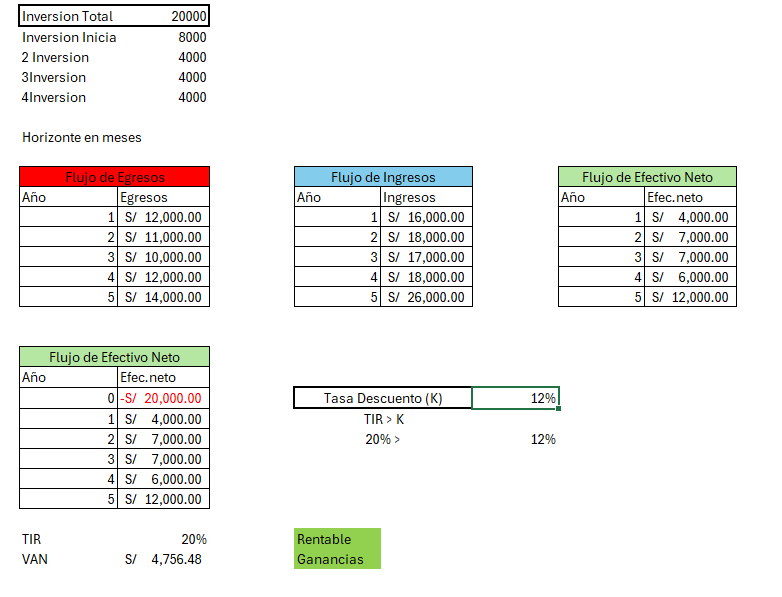
\includegraphics[width=1\textwidth]{van tir.png} % Imagen de ejemplo que viene con distribuciones LaTeX
    \label{fig:VAN Y TIR} % Etiqueta para referenciar la imagen en texto
    \textbf{Nota.} \textit{con un VAN de 4756.48 y un TIR del 20\%.}
\end{figure}

%inicio del capitulo 2 ---------------------------------------------------------------------------

\section*{\makebox[\linewidth][c]{Capítulo II}}
\addcontentsline{toc}{section}{Capítulo II}

\subsection*{Marco teórico}
\addcontentsline{toc}{subsection}{Marco teórico}

Los sistemas de inventario son herramientas clave para administrar con precisión los bienes y productos de una organización. Controlan entradas y salidas, mantienen registros al día y aseguran la disponibilidad.

\subsubsection*{Inventario periódico}
\addcontentsline{toc}{subsubsection}{Inventario periódico}

Se actualiza en intervalos definidos (semanal, mensual). Es simple y barato, pero no refleja el stock en tiempo real ni detecta quiebres a tiempo.

\subsubsection*{Inventario permanente o automatizado}
\addcontentsline{toc}{subsubsection}{Inventario permanente o automatizado}

Registra cada movimiento en el momento (ventas, compras, devoluciones, transferencias). Es ideal para múltiples sedes y alto volumen, mejora la trazabilidad y la toma de decisiones.

\subsection*{Antecedentes}
\addcontentsline{toc}{subsection}{Antecedentes}


%aqui falta


\subsection*{Metodología de Desarrollo}
\addcontentsline{toc}{subsection}{Metodología de Desarrollo}



Scrum es una metodología ágil e iterativa basada en la empiricidad (transparencia, inspección y adaptación). El trabajo se organiza en sprints de 1 a 4 semanas, al final de los cuales se entrega un incremento funcional y potencialmente desplegable. Los roles clave son Product Owner (prioriza valor), Scrum Master (facilita y remueve impedimentos) y un equipo multidisciplinario autoorganizado. Se apoya en eventos fijos —Sprint Planning, Daily, Review y Retrospective— y en artefactos como el Product Backlog y la Definición de Hecho; las historias de usuario guían el desarrollo y la revisión continua ajusta el rumbo.

\begin{itemize}
  \item Elementos clave:
  \begin{itemize}
    \item Historias de usuario: Describen funcionalidades desde la perspectiva del cliente.
    \item Criterios de aceptación: Definen cuándo una historia se considera completa.
    \item Sprint backlog: Lista de tareas a desarrollar en cada sprint.
    \item MVP (Producto Mínimo Viable): Versión inicial funcional que permite validar la solución con usuarios reales.
  \end{itemize}
\end{itemize}

\begin{figure}[h]
    \centering
    \caption{Carta gantt}
    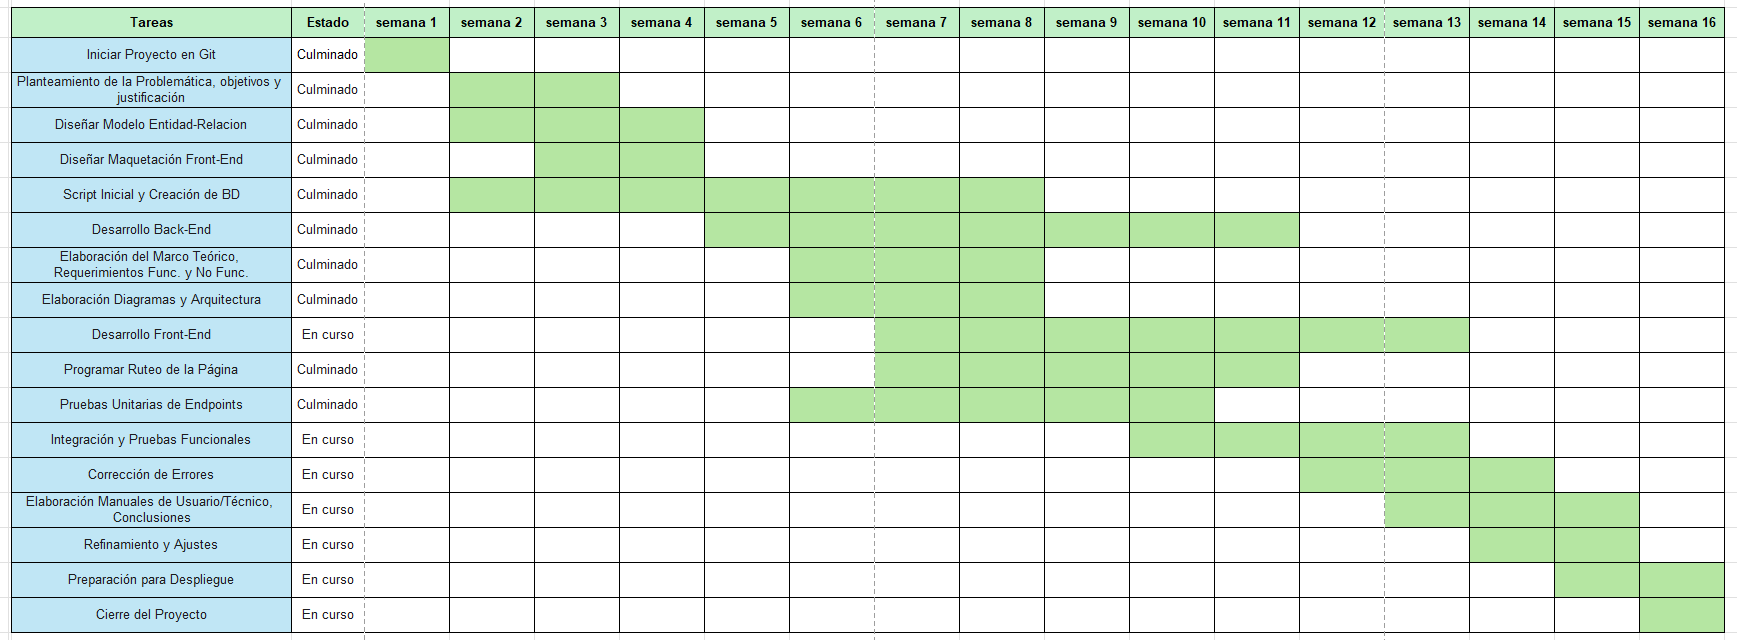
\includegraphics[width=1\textwidth]{gant2.png} % Imagen de ejemplo que viene con distribuciones LaTeX
    \textbf{Nota.} \textit{La carta Gantt muestra la planificación del proyecto durante 16 semanas}
\end{figure}

\subsection*{Diagrama de base}
\addcontentsline{toc}{subsection}{Diagrama de base}

\begin{figure}[H]
    \centering
    \caption{base de datos}
    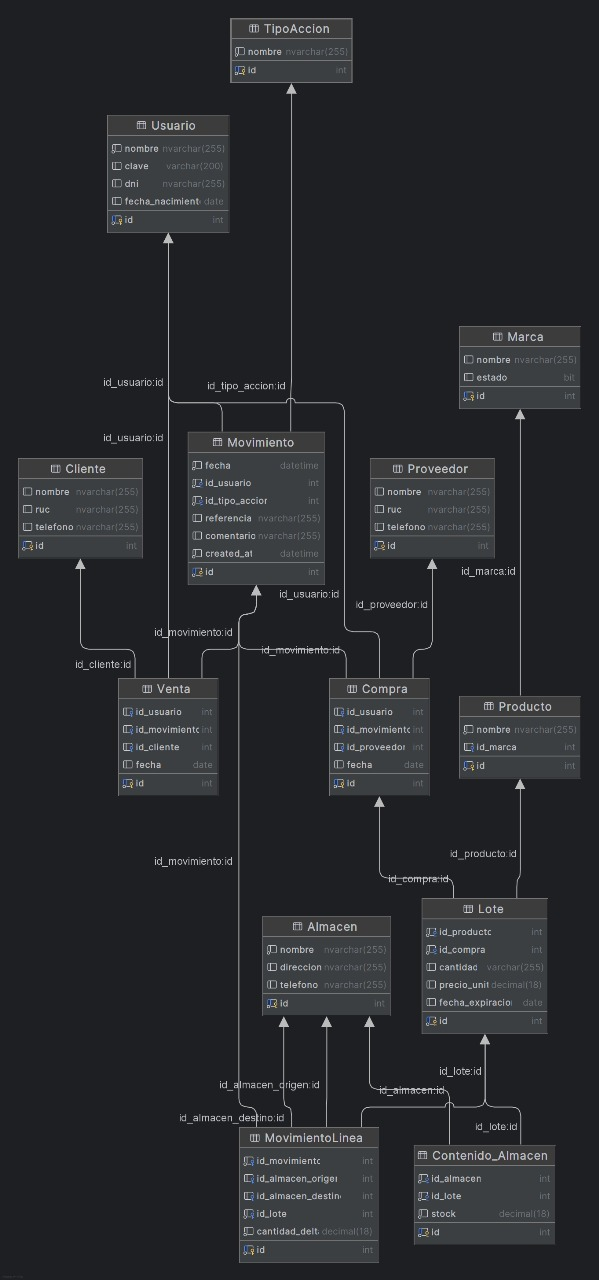
\includegraphics[width=0.6\textwidth]{Imagen de WhatsApp 2025-09-09 a las 11.22.15_6ae292d4.jpg}\\ % Imagen de ejemplo que viene con distribuciones LaTeX
    \vspace{0.5em}
    \textit{Representación de la estructura de la base de datos}
\end{figure}



\section*{\makebox[\linewidth][c]{Capítulo III}}
\addcontentsline{toc}{section}{Capítulo III}

\subsection*{Requerimientos}
\addcontentsline{toc}{subsection}{Requerimientos}

\subsubsection*{Funcionales}
\addcontentsline{toc}{subsubsection}{Funcionales}

Los requerimientos funcionales especifican las acciones y comportamientos que un sistema debe realizar para cumplir con las necesidades del usuario y los objetivos del negocio. Definen las tareas, procesos y funciones que el software debe ejecutar, como la gestión de datos, interacciones con el usuario o respuestas ante eventos. Son esenciales para guiar el desarrollo y la validación del sistema, asegurando que cumpla con lo esperado y facilite la comunicación entre equipos y usuarios, evitando malentendidos durante el proyecto.

\thispagestyle{plain}
  \footnotesize % Reduce aún más el tamaño de la fuente
  \renewcommand{\arraystretch}{3} % Reduce la altura de las filas
  
  % Ajustar el tamaño con adjustbox
  \begin{adjustbox}{width=\linewidth}
    \begin{tabularx}{\linewidth}{|>{\centering\arraybackslash}p{1cm}|
      >{\centering\arraybackslash}p{1.3cm}|
      >{\centering\arraybackslash}p{4.3cm}|
      >{\centering\arraybackslash}p{2.2cm}|
      >{\centering\arraybackslash}p{3.5cm}|
      >{\centering\arraybackslash}p{1.55cm}|}
\hline
      \rowcolor{headerbg} % Color de encabezado
      \textbf{ID} & \textbf{Nombre} & \textbf{Descripción} & \textbf{Rol de usuario} & \textbf{Criterios de aceptación} & \textbf{Prioridad}\\
      \hline
      RF-01 & Crear usuario & Permite registrar un nuevo usuario ingresando nombre, DNI y fecha de nacimiento & Administrador & El usuario se almacena correctamente y es visible en la lista & Alta\\
      \hline
      RF-02 & Editar usuario & Permite modificar los datos de un usuario existente & Administrador & Los cambios se reflejan al consultar el usuario & Alta\\
      \hline
      RF-03 & Eliminar usuario & Permite borrar un usuario & Administrador & El usuario ya no aparece en la lista & Media\\
      \hline
      RF-04 & Listar usuarios & Muestra los usuarios registrados con opción de búsqueda & Administrador & La búsqueda filtra correctamente & Alta\\
      \hline
      RF-05 & Crear cliente & Permite registrar un nuevo cliente con nombre, RUC y teléfono & Administrativo & El cliente aparece en la lista general & Alta \\
      \hline
      RF-06 & Editar cliente & Permite modificar los datos de un cliente existente & Administrativo & Cambios se muestran en la consulta & Alta \\
      \hline
      RF-07 & Eliminar cliente & Permite dar de baja un cliente & Administrativo & El cliente ya no figura en búsquedas & Media \\
      \hline
    \end{tabularx}
  \end{adjustbox}
  \normalsize


  \thispagestyle{plain}
  \footnotesize % Reduce aún más el tamaño de la fuente
  \renewcommand{\arraystretch}{3} % Reduce la altura de las filas
  
  % Ajustar el tamaño con adjustbox
  \begin{adjustbox}{width=\linewidth}
    \begin{tabularx}{\linewidth}{|>{\centering\arraybackslash}p{1cm}|
      >{\centering\arraybackslash}p{1.3cm}|
      >{\centering\arraybackslash}p{4.3cm}|
      >{\centering\arraybackslash}p{2.2cm}|
      >{\centering\arraybackslash}p{3.5cm}|
      >{\centering\arraybackslash}p{1.55cm}|}
\hline
      RF-08 & Listar clientes & Visualiza los clientes registrados y permite buscarlos & Administrativo & Filtros y listados funcionales & Alta \\
      \hline
      RF-09 & Crear proveedor & Permite registrar proveedores nuevos con nombre, RUC y teléfono & Administrativo & El proveedor se visualiza en la lista general & Media \\
      \hline
      RF-10 & Editar proveedor & Permite editar información de proveedores existentes & Administrativo & Cambios son validados y almacenados & Media \\
      \hline
      RF-11 & Eliminar proveedor & Permite eliminar un proveedor del sistema & Administrativo & El proveedor es eliminado de la lista & Baja \\
      \hline
      RF-12 & Listar proveedores & Muestra y filtra la lista de proveedores registrados & Administrativo & Se pueden buscar proveedores existentes & Media \\
      \hline
      RF-13 & Crear almacén & Permite registrar un nuevo almacén & Administrador & El almacén se almacena correctamente & Alta \\
      \hline
      RF-14 & Gestionar productos y marcas & Permite creación, modificación y eliminación de productos y marcas & Administrativo & Operaciones se ejecutan satisfactoriamente & Alta \\
      \hline
      
    \end{tabularx}
  \end{adjustbox}
  \normalsize

  \thispagestyle{plain}
  \footnotesize % Reduce aún más el tamaño de la fuente
  \renewcommand{\arraystretch}{3} % Reduce la altura de las filas
  
  % Ajustar el tamaño con adjustbox
  \begin{adjustbox}{width=\linewidth}
    \begin{tabularx}{\linewidth}{|>{\centering\arraybackslash}p{1cm}|
      >{\centering\arraybackslash}p{1.3cm}|
      >{\centering\arraybackslash}p{4.3cm}|
      >{\centering\arraybackslash}p{2.2cm}|
      >{\centering\arraybackslash}p{3.5cm}|
      >{\centering\arraybackslash}p{1.55cm}|}
\hline
      RF-15 & Registrar lote & Permite registrar un lote para un producto y compra específica & Administrativo & El lote queda vinculado a su producto y compra & Alta \\
      \hline
      RF-16 & Controlar inventario & Registra y actualiza stock de lotes en los almacenes, mostrando cantidades actuales & Administrador & El stock es exacto y se actualiza en base a movimientos registrados & Alta \\
      \hline
      RF-17 & Registrar movimiento & Permite el registro de entrada, salida o traslado entre almacenes & Operador & El movimiento genera el ajuste esperado en los participantes & Alta \\
      \hline
      RF-18 & Consultar movimientos & Listar todos los movimientos realizados, filtrando por fechas, usuario y tipo & Administrador & Filtros retornan resultados adecuados & Media \\
      \hline
      RF-19 & Registrar compra & Permite almacenar información de una compra y asociarla a proveedor y lotes & Administrativo & Compra queda grabada y relacionada con lotes y proveedor & Alta \\
      \hline
      RF-20 & Registrar venta & Permite almacenar información de una venta y asociarla a cliente y movimientos & Administrativo & Venta queda registrada y asocia los datos correspondientes & Alta \\
      \hline
    \end{tabularx}
  \end{adjustbox}
  \normalsize

\subsubsection*{No Funcionales}
\addcontentsline{toc}{subsubsection}{No Funcionales}

Los requerimientos no funcionales definen cómo debe comportarse un sistema, abordando aspectos como seguridad, rendimiento y usabilidad. Son clave para garantizar su calidad, confiabilidad y una buena experiencia de usuario, por lo que no deben pasarse por alto.

\thispagestyle{plain}
  \footnotesize % Reduce aún más el tamaño de la fuente
  \renewcommand{\arraystretch}{3} % Reduce la altura de las filas
  
  % Ajustar el tamaño con adjustbox
  \begin{adjustbox}{width=\linewidth}
    \begin{tabularx}{\linewidth}{|>{\centering\arraybackslash}p{1.3cm}|
      >{\centering\arraybackslash}p{2.1cm}|
      >{\centering\arraybackslash}p{5.1cm}|
      >{\centering\arraybackslash}p{4.1cm}|
      >{\centering\arraybackslash}p{1.7cm}|}
\hline
      \rowcolor{headerbg} % Color de encabezado
      \textbf{ID} & \textbf{Categoría} & \textbf{Descripción} & \textbf{Criterio de aceptación} & \textbf{Prioridad}\\
      \hline
      RNF-01 & Seguridad & El sistema debe requerir autenticación para acceder a todas las funcionalidades. & Ningún usuario no autenticado puede acceder a la aplicación & Alta \\
      \hline
      RNF-02 & Seguridad & Los datos personales deben almacenarse cifrados. & La base de datos almacena información sensible encriptada & Alta \\
      \hline
      RNF-03 & Rendimiento & El tiempo de respuesta ante consultas de usuarios no debe superar 2 segundos en el 95\% de los casos. & Reportes de uso muestran cumplimiento del estándar & Alta \\
      \hline
      RNF-04 & Disponibilidad & El sistema debe estar disponible el 99.5\% del tiempo en horario laboral. & Logs de uptime validan el cumplimiento & Media \\
      \hline
      RNF-05 & Usabilidad & La interfaz debe ser intuitiva y accesible para usuarios nuevos, con mensajes claros de error y éxito. & Encuestas de satisfacción mayores a 80\% en pruebas & Media \\
      \hline
      RNF-06 & Escalabilidad & El sistema debe soportar ampliación a más almacenes y usuarios sin degradar el rendimiento. & Pruebas de carga mantienen rendimiento aceptable & Media \\
      \hline
    \end{tabularx}
  \end{adjustbox}
  \normalsize

  \thispagestyle{plain}
  \footnotesize % Reduce aún más el tamaño de la fuente
  \renewcommand{\arraystretch}{3} % Reduce la altura de las filas
  
  % Ajustar el tamaño con adjustbox
  \begin{adjustbox}{width=\linewidth}
    \begin{tabularx}{\linewidth}{|>{\centering\arraybackslash}p{1.3cm}|
      >{\centering\arraybackslash}p{2.3cm}|
      >{\centering\arraybackslash}p{5.1cm}|
      >{\centering\arraybackslash}p{4.1cm}|
      >{\centering\arraybackslash}p{1.5cm}|}
\hline
      RNF-07 & Mantenibilidad & El sistema debe documentar su código y procesos clave para facilitar su actualización y corrección. & Manual técnico y comentarios obligatorios en el código & Media \\
      \hline
      RNF-08 & Compatibilidad & Debe funcionar correctamente en los navegadores modernos (Chrome, Firefox, Edge). & Pruebas de compatibilidad con los principales navegadores & Baja \\
      \hline
      RNF-09 & Backup & Debe ser posible restaurar la información mediante backups automáticos diarios. & Simulacros de recuperación de datos correctos & Media \\
      \hline
    \end{tabularx}
  \end{adjustbox}
  \normalsize

\subsection*{Metodología de desarrollo desplegada}
\addcontentsline{toc}{subsection}{Metodología de desarrollo desplegada}

Para lograr una buena gestión y ejecución del proyecto, se adoptó la metodología de desarrollo \textbf{scrum}. El cual, se fundamenta en en un enfoque ágil e iterativo que promueve la entrega incremental de valor, la colaboración constante entre los miembros del equipo y la adaptación continua a los cambios. Esta metodología divide el trabajo en ciclos cortos llamados \textit{Sprints}, en los que se planifican, desarrollan y revisan funcionalidades del producto de manera continua, asegurando así una mejora constante y una mayor satisfacción del cliente.

Se definieron los roles dentro del equipo y se implementaron los eventos característicos de Scrum, tales como:

\begin{itemize}
  \item \textbf{Sprint Backlog}: Es el trabajo a realizar durante un sprint, definido durante las reuniónes de Planificación de Sprint. Incluye el objetivo del Sprint (\textit{Sprint Goal}) y los elementos del Product Backlog seleccionados para ser completados en ese sprint.

  \item \textbf{Sprint}: Planificación de 1 semana en el que se desarrollaron ideas y se convierten en valor.

  \item \textbf{Planificación de Sprint}: En esta reunión se definieron los objetivos del Sprint y el trabajo a realizar durante el sprint. Por lo que, la duración de esta reunión duro en total 336.

  \item \textbf{Scrum Diario}: La reunión durara alrededor de 15 minutos y sera realizada diariamente a la misma hora con el Equipo de Desarrollo para agilizar el proceso de desarrollo.

  \item \textbf{Revisión de Sprint}: Esta reunión tiene una duración máxima de 4 horas para sprints de un mes.
\end{itemize}

\subsection*{Diagrama de clases}
\addcontentsline{toc}{subsection}{Diagrama de clases}


\begin{figure}[H]
    \centering
    \caption{Diagrama de clases}
    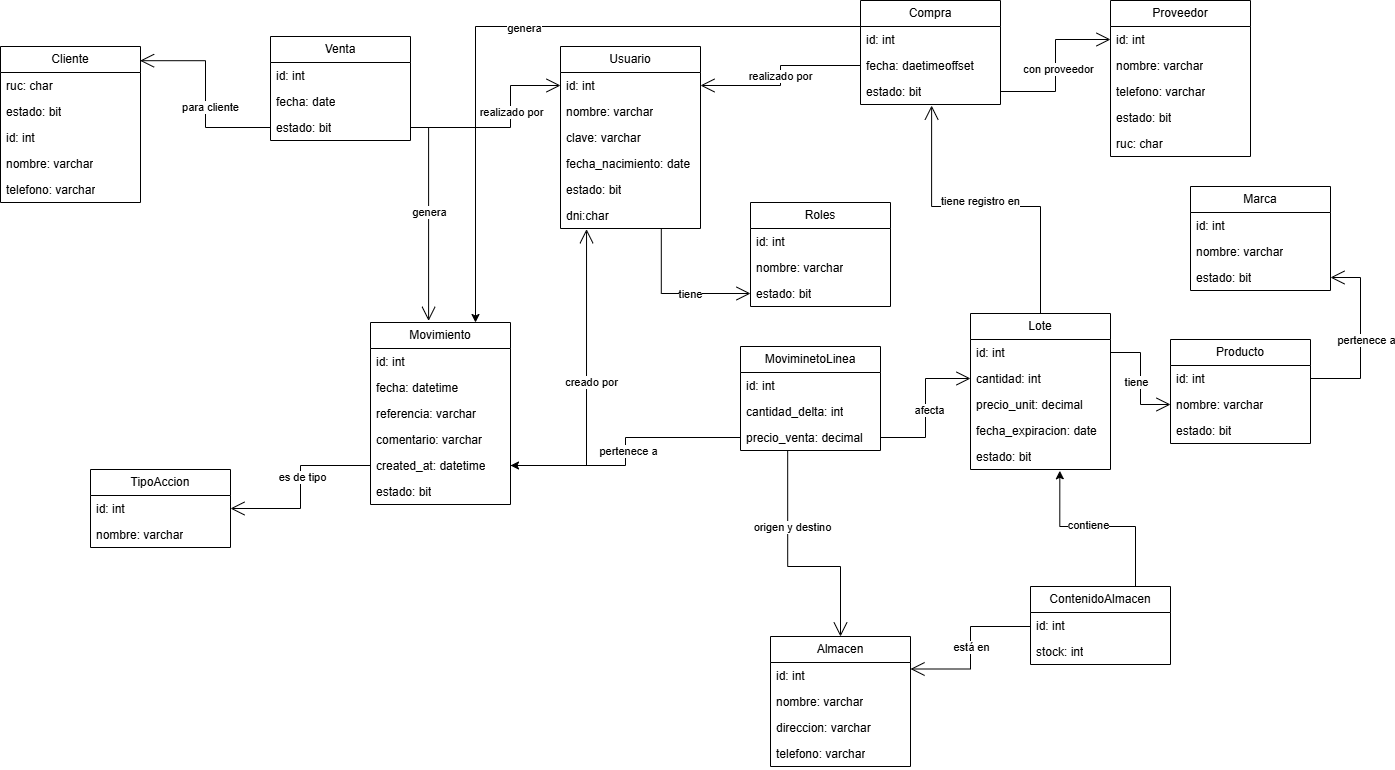
\includegraphics[width=0.9\textwidth]{diagrama de clases.png}\\ % Imagen de ejemplo que viene con distribuciones LaTeX
    \vspace{0.5em}
    \textit{Diagrama UML de clases que representa la estructura y relaciones entre los objetos del sistema.}
\end{figure}

\begin{description}

  \item[Entidades Maestras (Catálogos):] Son las clases que almacenan datos centrales que rara vez cambian.
    \begin{description}
      \item[Usuario:] Gestiona las cuentas que acceden al sistema, sus credenciales y su Rol.

      \item[Cliente:] Almacena la información de los compradores (\texttt{RUC}, nombre).

      \item[Proveedor:] Almacena los datos de los proveedores (\texttt{RUC}, nombre).

      \item[Producto:] Es el artículo físico a inventariar (nombre), asociado a una \textbf{Marca}.

      \item[Almacén:] Representa las ubicaciones físicas (dirección, teléfono) donde se guarda el stock.
    \end{description}

  \item[Entidades Transaccionales (Procesos):] Son las clases que registran las operaciones del negocio.
    \begin{description}
      \item[Compra y Venta:] Son los procesos de negocio. Una \textbf{Venta} se asocia a un \textbf{Cliente} y una \textbf{Compra} a un \textbf{Proveedor}. Ambas son realizadas por un \textbf{Usuario} y, fundamentalmente, ambas generan un \textbf{Movimiento}.

      \item[Movimiento:] Es el corazón del inventario. Actúa como un registro central de todas las operaciones (entradas, salidas, traslados). Es creado por un \textbf{Usuario} y se clasifica según un \textbf{TipoAccion} %(ej. \textit{"Entrada por Compra"}, \textit{"Salida por Venta"}).
    \end{description}

  \item[Entidades de Inventario (Detalle):] Son las clases que conectan los productos con las transacciones y el stock.
    \begin{description}
      \item[Lote:] El sistema gestiona el inventario por lotes. Cada \textbf{Lote} tiene un \texttt{precio\_unit} y \texttt{fecha\_expiracion}, y está relacionado con un \textbf{Producto}.

      \item[MovimientoLinea:] Es el detalle de un \textbf{Movimiento}. Especifica la cantidad de un \textbf{Lote} que se está moviendo.

      \item[ContenidoAlmacen:] Es la clase que representa el stock real. Conecta un \textbf{Almacén} con un \textbf{Lote} y almacena la cantidad física (\textit{stock}) disponible en esa ubicación.
    \end{description}

\end{description}



\subsection*{Diagrama de base de datos}
\addcontentsline{toc}{subsection}{Diagrama de base de datos}


\begin{figure}[H]
    \centering
    \caption{Diagrama de la base de datos}
    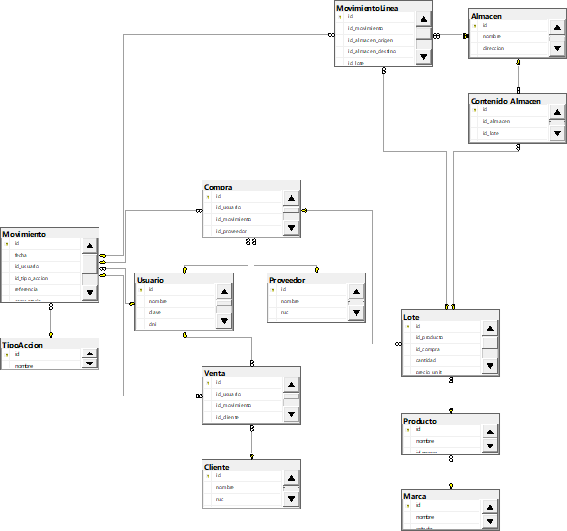
\includegraphics[width=1\textwidth]{diagrama base.png}\\ % Imagen de ejemplo que viene con distribuciones LaTeX
    \vspace{0.5em}
    \textit{Diagrama que muestra la estructura de la base de datos y las relaciones entre tablas.}
\end{figure}



\subsection*{Diseño de entorno}
\addcontentsline{toc}{subsection}{Diseño de entorno}

Para el presente proyecto, se ha implementado una Arquitectura de 5 Capas, un modelo robusto que separa las responsabilidades del sistema en cinco niveles lógicos distintos: Modelo, Repositorio, Servicio, Controlador, y Configuración.

\begin{figure}[H]
    \centering
    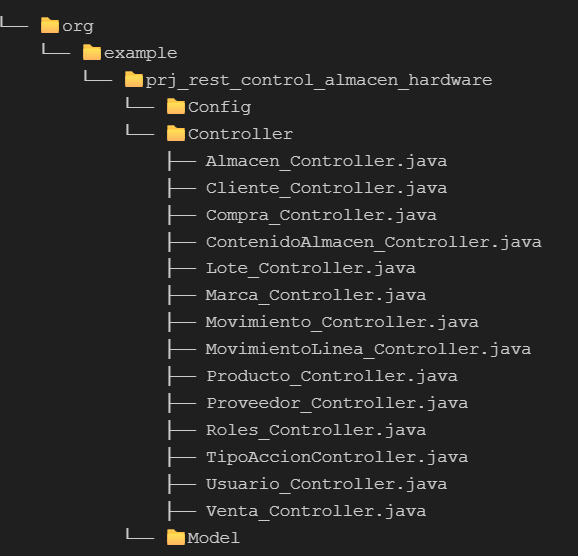
\includegraphics[width=1\textwidth]{entor1.png} % Imagen de ejemplo que viene con distribuciones LaTeX
\end{figure}

\begin{figure}[H]
    \centering
    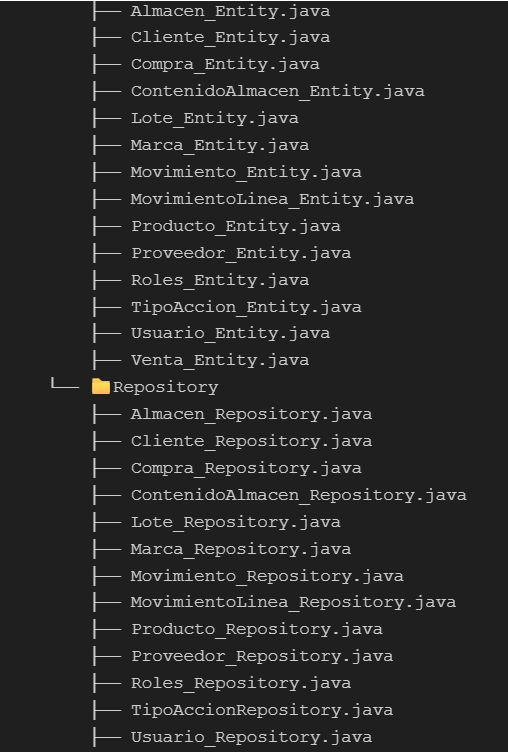
\includegraphics[width=1\textwidth]{entor2.png} % Imagen de ejemplo que viene con distribuciones LaTeX
\end{figure}

\begin{figure}[H]
    \centering
    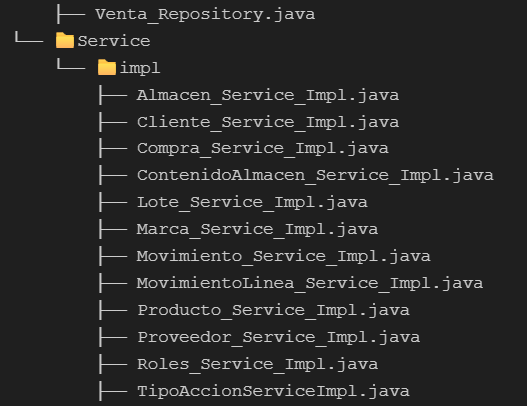
\includegraphics[width=0.8\textwidth]{entor3.png} % Imagen de ejemplo que viene con distribuciones LaTeX
\end{figure}

\begin{figure}[H]
    \centering
    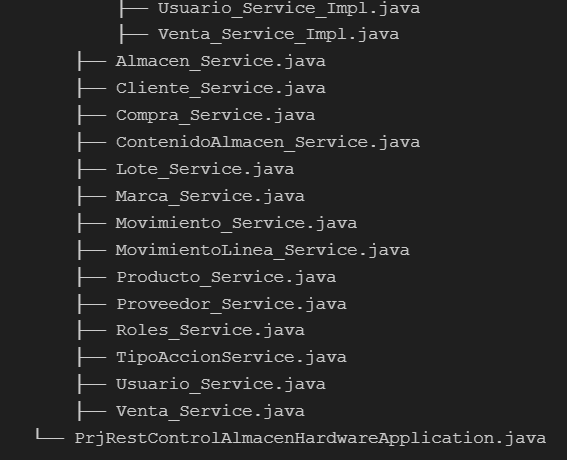
\includegraphics[width=0.8\textwidth]{entor4.png} % Imagen de ejemplo que viene con distribuciones LaTeX
\end{figure}

El proyecto utiliza una arquitectura en capas que sirve como base, la cual se ha adaptado específicamente para el desarrollo de APIs REST siguiendo el patrón Model-View-Controller (MVC). En este enfoque, la función tradicional de la "Vista" en MVC se reemplaza por la generación de respuestas en formato JSON, adecuándose así a la naturaleza de las APIs.

La implementación de esta arquitectura se basa en una clara separación de responsabilidades, donde cada capa cumple un rol específico y bien definido. Esto facilita la organización del proyecto, así como el mantenimiento y las pruebas del código.

\subsubsection*{Estructura y Patrones de Diseño Aplicados}
\addcontentsline{toc}{subsubsection}{Estructura y Patrones de Diseño Aplicados}

La estructura del proyecto se divide en las siguientes capas, aplicando patrones de diseño específicos:

\begin{itemize}
  \item \textbf{Capa de Modelo (Model):}  
  Se encarga de representar las entidades de la base de datos como objetos Java. Para ello, utiliza el patrón Entity, mediante clases anotadas con JPA (\texttt{@Entity}), que mapean directamente las tablas en SQL Server y contienen únicamente la estructura de los datos.

  \item \textbf{Capa de Repositorio (Repository):}  
  Proporciona el acceso directo a la base de datos para realizar operaciones CRUD (Crear, Leer, Actualizar y Eliminar). Esta capa aplica el patrón Repository, implementado mediante interfaces que extienden \texttt{JpaRepository}, lo que abstrae la lógica de persistencia y permite manipular los datos sin exponer los detalles de la base a otras capas.

  \item \textbf{Capa de Servicio (Service):}  
  Aquí se encuentra la lógica de negocio: se realizan validaciones y se coordinan las operaciones necesarias llamando a los repositorios. Se aplica el patrón Service Layer, complementado con la inyección de dependencias (\textit{Dependency Injection}) mediante \texttt{@Autowired} para integrar los repositorios requeridos.

  \item \textbf{Capa de Controlador (Controller):}  
  Funciona como la interfaz de comunicación del sistema. Recibe las solicitudes HTTP externas, las dirige a la capa de servicio correspondiente y construye las respuestas HTTP. Emplea el patrón Controller, usando anotaciones de Spring Boot (\texttt{@RestController}, \texttt{@GetMapping}, etc.) para exponer los endpoints REST.

  \item \textbf{Capa de Configuración (Config):}  
  Gestiona configuraciones globales y transversales del sistema, tales como la configuración CORS, la seguridad con JWT y la documentación de la API (Swagger). Se basa en el patrón Configuration, utilizando anotaciones como \texttt{@Configuration} y \texttt{@Bean} para definir elementos y componentes gestionados por el contenedor de Spring.
\end{itemize}

\subsubsection*{Dependencia e Inyección}
\addcontentsline{toc}{subsubsection}{Dependencia e Inyección}

La interacción entre las capas se gestiona de manera rigurosa mediante la Inyección de Dependencias que proporciona Spring Boot. Las dependencias fluyen en una sola dirección: el controlador depende del servicio, y el servicio depende del repositorio.

Esta arquitectura aporta varios beneficios clave para el desarrollo:

\begin{itemize}
  \item \textbf{Mantenibilidad:} Los cambios específicos, como modificaciones en la base de datos o en la lógica de negocio, afectan únicamente a la capa correspondiente sin propagarse innecesariamente al resto del sistema.

  \item \textbf{Testabilidad:} Cada capa puede ser probada de forma independiente mediante pruebas unitarias, facilitando la identificación y corrección de errores.

  \item \textbf{Escalabilidad y reutilización:} Es sencillo incorporar nuevas funcionalidades, y la lógica de negocio contenida en los servicios puede ser reutilizada por múltiples controladores.

  \item \textbf{Claridad:} La estructura de carpetas refleja intuitivamente la separación de responsabilidades, lo que mejora la comprensión y el mantenimiento del código.
\end{itemize}

\subsection*{Codificacion}
\addcontentsline{toc}{subsection}{Codificacion}

\subsubsection*{Capa de Modelo}
\addcontentsline{toc}{subsubsection}{Capa de Modelo}

\begin{figure}[H]
    \centering
    \caption{MovimientoLinea}
    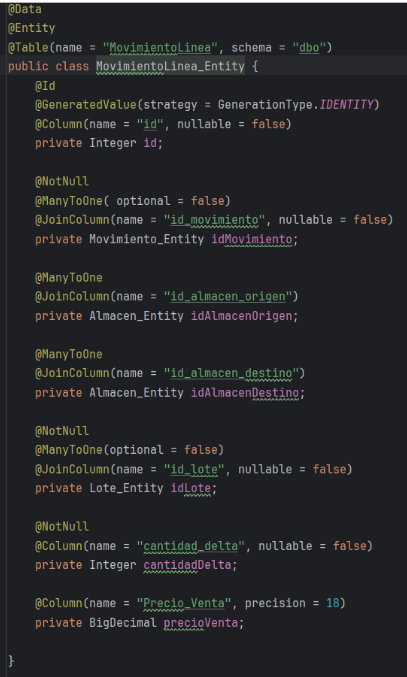
\includegraphics[width=0.7\textwidth]{mode1.png}\\ % Imagen de ejemplo que viene con distribuciones LaTeX
    \textit{Modelo backend correspondiente a la entidad \textit{MovimientoLinea\_Entity}.}
\end{figure}



La Capa de Modelo representa el núcleo de la persistencia de datos. Su función principal es mapear la tabla física de la base de datos (\texttt{MovimientoLinea}) a un objeto Java (\texttt{MovimientoLinea\_Entity}), aplicando el patrón Entity con anotaciones JPA. Esta capa define la estructura de la entidad, que incluye una clave primaria autoincrementada, y utiliza anotaciones de Lombok para minimizar el código repetitivo, como getters y setters.

Además, gestiona las relaciones \textit{uno a muchos} y \textit{muchos a uno} (\texttt{@ManyToOne}), conectando la línea de movimiento con entidades clave como \texttt{Movimiento}, \texttt{Lote} y los almacenes de origen y destino. Esto asegura la integridad referencial y permite una carga eficiente de los datos relacionados dentro de la aplicación.

\subsubsection*{Capa de Repositorio}
\addcontentsline{toc}{subsubsection}{Capa de Repositorio}

\begin{figure}[H]
    \centering
    \caption{MovimientoLineaRepository}
    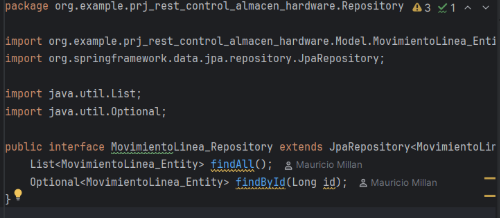
\includegraphics[width=0.7\textwidth]{repo1.png}\\ % Imagen de ejemplo que viene con distribuciones LaTeX
    \textit{Repositorio backend correspondiente a la entidad \textit{MovimientoLinea\_Entity}.}
\end{figure}

La Capa de Repositorio actúa como el enlace exclusivo entre la Capa de Servicio y la base de datos, implementando el patrón Repository. Su principal función es abstraer la lógica de persistencia, aislando así a la Capa de Servicio de los detalles específicos de las consultas SQL.

Al extender la interfaz \texttt{JpaRepository}, esta capa hereda automáticamente los métodos CRUD básicos (como \texttt{save}, \texttt{findById}, \texttt{findAll} y \texttt{deleteById}) para la entidad \texttt{MovimientoLinea\_Entity}, sin necesidad de escribir código SQL manual. Esto permite que el servicio obtenga datos mediante interfaces simples (por ejemplo, \texttt{repository.findAll()}) sin preocuparse por la complejidad de la sintaxis SQL.

\subsubsection*{Capa de Servicio}
\addcontentsline{toc}{subsubsection}{Capa de Servicio}

\begin{figure}[H]
    \centering
    \caption{MovimientoLineaService}
    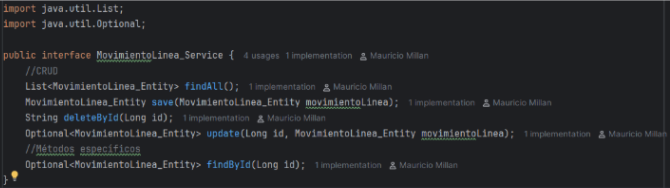
\includegraphics[width=0.7\textwidth]{servi1.png}\\ % Imagen de ejemplo que viene con distribuciones LaTeX
\end{figure}

\begin{figure}[H]
    \centering
    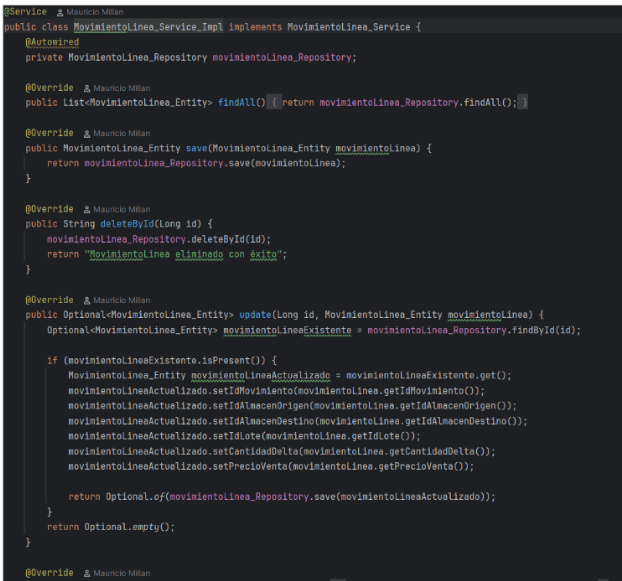
\includegraphics[width=0.8\textwidth]{servi2.png}\\ % Imagen de ejemplo que viene con distribuciones LaTeX
    \textit{Servicio backend correspondiente a la entidad \textit{MovimientoLinea\_Entity}.}
\end{figure}

La Capa de Servicio es el motor de la lógica de negocio y la orquestación, siguiendo el patrón Service Layer. Su principal responsabilidad es centralizar todas las reglas, validaciones y cálculos antes de que los datos sean guardados o retornados. Por ejemplo, en esta capa se debe validar que el \textit{cantidadDelta} de un producto no provoque un stock negativo, o calcular automáticamente el precio de venta.

La implementación del servicio utiliza la inyección de dependencias (\texttt{@Autowired}) para acceder al Repositorio y realiza las operaciones básicas como listar, guardar, actualizar y eliminar, tal como se definen en su interfaz. Esto garantiza una separación clara entre la lógica de negocio y la capa de acceso a datos.


\subsubsection*{Capa de Controlador}
\addcontentsline{toc}{subsubsection}{Capa de Controlador}

\begin{figure}[H]
    \centering
    \caption{MovimientoLineaController}
    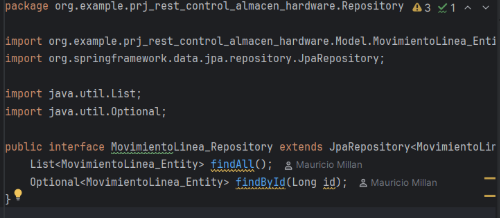
\includegraphics[width=0.7\textwidth]{repo1.png}\\ % Imagen de ejemplo que viene con distribuciones LaTeX
    \textit{Controller backend correspondiente a la entidad \textit{MovimientoLinea\_Entity}.}
\end{figure}

La Capa de Controlador es la puerta de entrada de la API, exponiendo los endpoints RESTful al exterior y aplicando el patrón Controller. Su función es manejar las solicitudes HTTP entrantes (como GET, POST, PUT, DELETE) en la ruta \texttt{/api/movimiento-lineas}. Utiliza la inyección de dependencias para acceder a la Capa de Servicio y delega en ella la ejecución de la lógica de negocio.

El controlador no contiene lógica de negocio; su tarea es recibir el JSON enviado por el cliente, invocar el método correspondiente en el servicio, y transformar el resultado de las entidades Java en una respuesta HTTP (JSON) con el código de estado adecuado (por ejemplo, 200 OK, 204 No Content, 404 Not Found).

El flujo de datos sigue la dirección de la inyección de dependencias (Controlador → Servicio → Repositorio): una petición HTTP llega al controlador, que pasa la validación y la lógica al servicio, este interactúa con el repositorio para ejecutar la consulta SQL, y el resultado regresa como una respuesta JSON al cliente.

Los patrones clave aplicados en la arquitectura son: Entity Pattern (JPA), Repository Pattern para la abstracción de datos, Service Layer Pattern para la lógica de negocio, y Dependency Injection que integra todas las capas.


\section*{anexos}
\addcontentsline{toc}{section}{anexos}

\begin{figure}[h]
    \centering
    \caption{Carta gantt}
    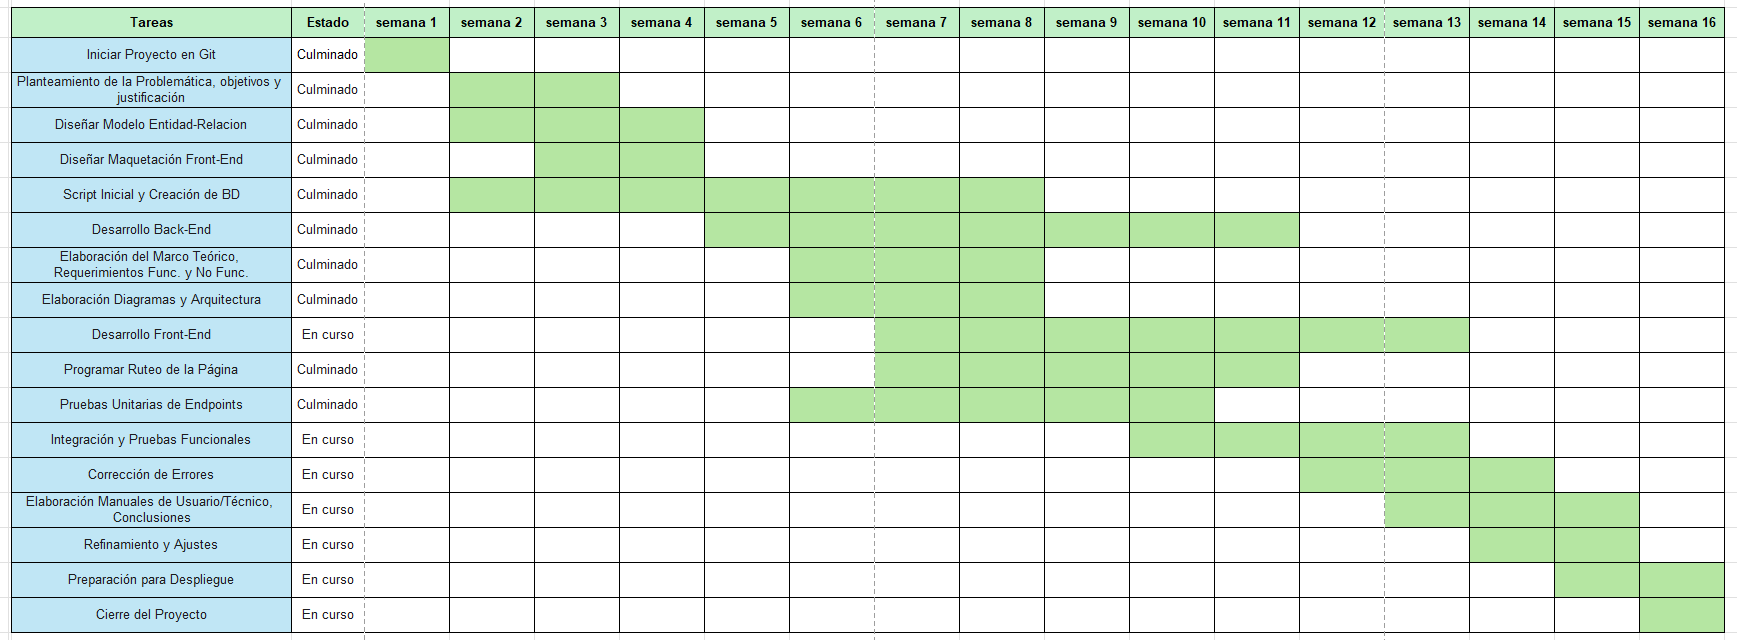
\includegraphics[width=1\textwidth]{gant2.png} % Imagen de ejemplo que viene con distribuciones LaTeX
    \textbf{Nota.} \textit{La carta Gantt muestra la planificación del proyecto durante 16 semanas}
\end{figure}

\begin{figure}[H]
    \centering
    \caption{base de datos}
    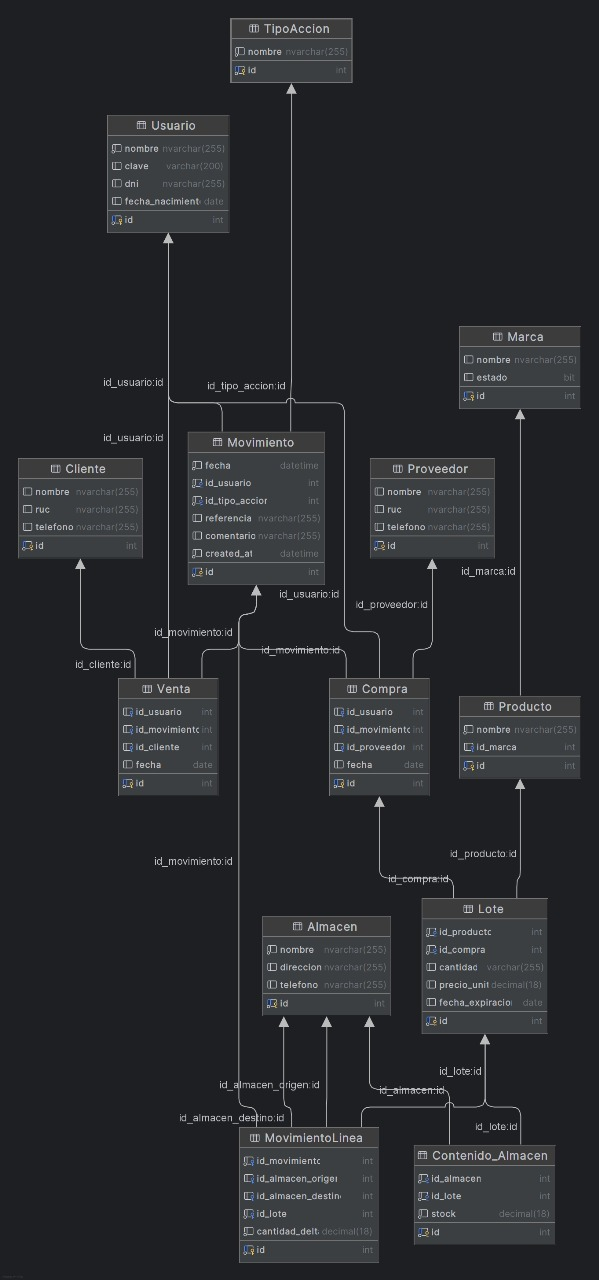
\includegraphics[width=0.6\textwidth]{Imagen de WhatsApp 2025-09-09 a las 11.22.15_6ae292d4.jpg}\\ % Imagen de ejemplo que viene con distribuciones LaTeX
    \vspace{0.5em}
    \textit{Representación de la estructura de la base de datos}
\end{figure}

\begin{figure}[H]
    \centering
    \caption{Diagrama de clases}
    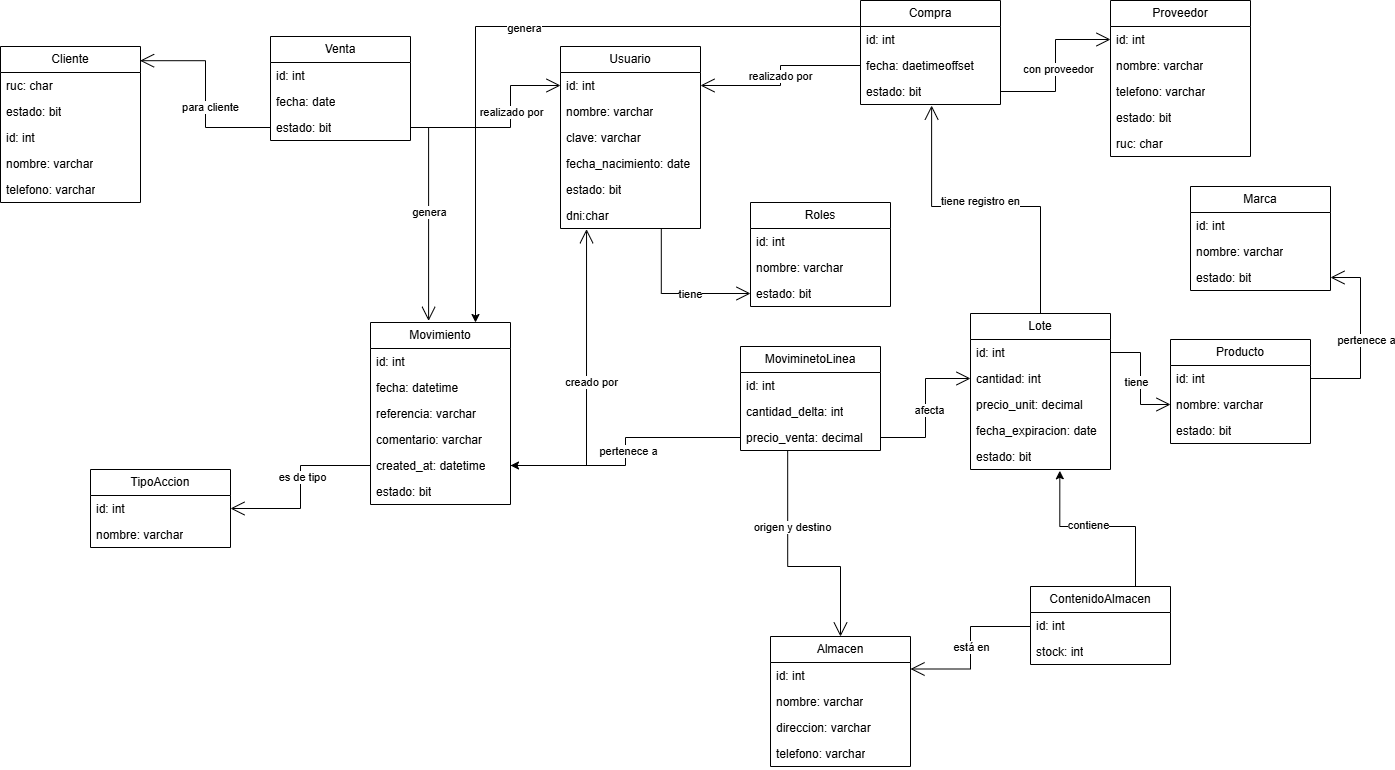
\includegraphics[width=0.9\textwidth]{diagrama de clases.png}\\ % Imagen de ejemplo que viene con distribuciones LaTeX
    \vspace{0.5em}
    \textit{Diagrama UML de clases que representa la estructura y relaciones entre los objetos del sistema.}
\end{figure}

\begin{figure}[H]
    \centering
    \caption{Diagrama de la base de datos}
    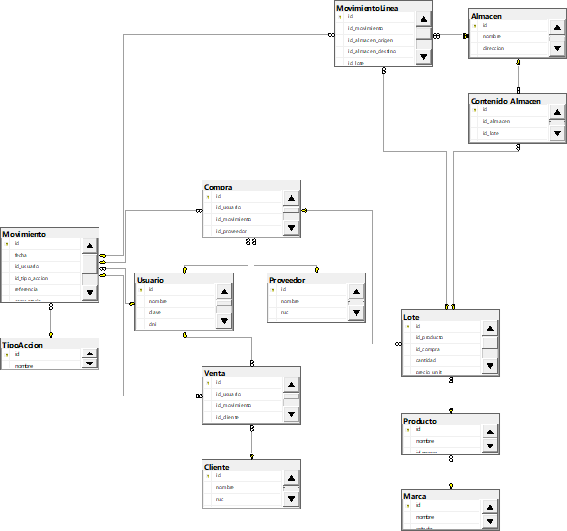
\includegraphics[width=1\textwidth]{diagrama base.png}\\ % Imagen de ejemplo que viene con distribuciones LaTeX
    \vspace{0.5em}
    \textit{Diagrama que muestra la estructura de la base de datos y las relaciones entre tablas.}
\end{figure}

% Muy pronto los demas capitulos...


\end{document}
